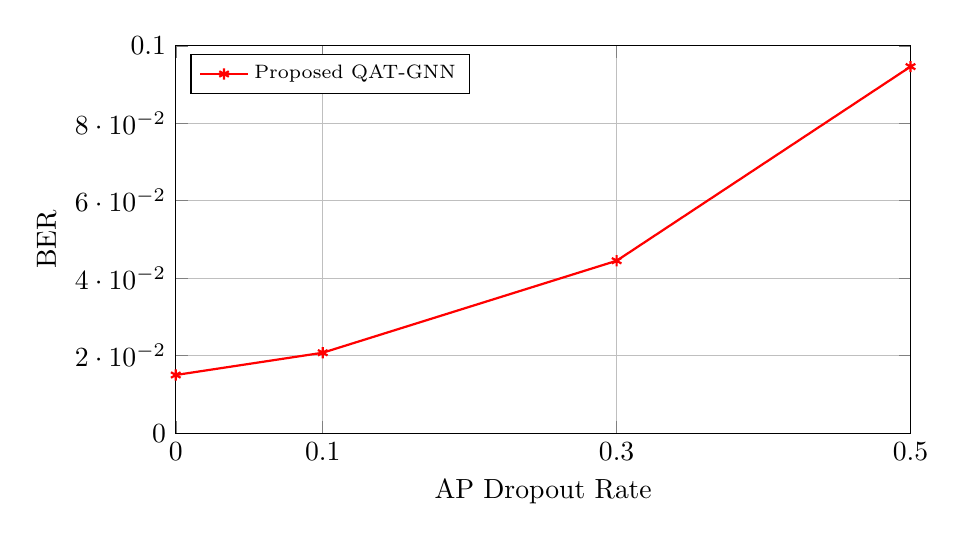
\begin{tikzpicture}
\begin{axis}[
    width=0.9\linewidth,
    height=6.5cm,
    xlabel={AP Dropout Rate},
    ylabel={BER},
    xmin=0, xmax=0.5,
    ymin=0, ymax=0.1,
    xtick={0,0.1,0.3,0.5},
    grid=both,
    legend style={at={(0.02,0.98)},anchor=north west,font=\scriptsize},
    legend cell align={left}
]
\addplot[color=red,mark=asterisk,thick] coordinates {
(0.0, 0.01500) (0.1, 0.02075) (0.3, 0.04450) (0.5, 0.09463)
};
\addlegendentry{Proposed QAT-GNN}

\end{axis}
\end{tikzpicture}